\documentclass[11pt]{article}
\usepackage{paper_style}
\usepackage{graphicx} % Required for inserting images
\usepackage{indentfirst}
\usepackage{lipsum}
\usepackage{array}
\usepackage{float}
\usepackage{longtable}
\usepackage{enumitem}
\usepackage{hyperref}
\usepackage{float}
\usepackage{censor}
\usepackage{tabularx}
\usepackage[noabbrev,capitalize]{cleveref}
\usepackage{amsmath}

%% ===============================================
%% Setting the line spacing (3 options: only pick one)
% \doublespacing
% \singlespacing
\onehalfspacing
%% ===============================================

\setlength{\droptitle}{-5em} %% Don't touch

\newcommand{\zerodisplayskips}{%
  \setlength{\abovedisplayskip}{0pt}%
  \setlength{\belowdisplayskip}{5pt}%
  \setlength{\abovedisplayshortskip}{0pt}%
  \setlength{\belowdisplayshortskip}{5pt}}
\appto{\normalsize}{\zerodisplayskips}
\appto{\small}{\zerodisplayskips}
\appto{\footnotesize}{\zerodisplayskips}

\renewcommand\tabularxcolumn[1]{m{#1}}
\crefname{section}{Section}{Sections}
\crefname{figure}{Figure}{Figures}
\creflabelformat{equation}{#2\textup{#1}#3}

\newcolumntype{C}[1]{>{\centering\arraybackslash}p{#1}}

\title{Investigation of the Relationship between Temperature and Equilibrium Constant of a Thiocyanatoiron Complex Reaction}
\author{\censor{Saptak Das}}
\date{January 2023}

\begin{document}

\maketitle

\section{Introduction}
\label{section:introduction}
As someone who wants to major in Control Theory, the field of engineering that deals with the control of dynamic systems and processes, I have always been fascinated by industrial chemical processes like the Haber-Bosch Process and the Fischer-Tropsch Process. Specifically, I have always wondered how chemical engineers have optimized the efficiency and yield of these processes by selectively choosing the temperature and pressure conditions for the reaction.

In my chemistry class, I learned about how Le Chatelier’s principle could be applied to shift the chemical equilibrium towards a desired product. However, I soon realized that knowing which product is thermodynamically favored is only one factor among many such as reaction rate and practical feasibility that chemical engineers must consider. Chemical engineers must realize the relationship between the temperature and equilibrium constant to find the precise temperature compromise to precisely optimize for all such factors \citep{libretextsHaberProcess}. Hence, I decided to explore how temperature affects the equilibrium constant for a thiocyanatoiron complex reaction for my Chemistry Internal Assessment.


\subsection{Research Question}
\noindent
What is the relationship between the equilibrium constant and temperature of a thiocyanatoiron complex reaction?

\section{Background Research}
\subsection{Primary Reaction}
\noindent
This experiment will use the thiocyanatoiron complex reaction as a means to explore the relationship between the equilibrium constant and temperature. The complex formation reaction is described below \citep{buffalostateChemicalEquilibrium}.

\begin{equation*}
    Fe^{3+} + SCN^- \rightleftharpoons FeSCN^{2+}
\end{equation*}

\subsection{Equilibrium Constant}
The equilibrium constant (\(K_c\)) is a measure of the extent to which a chemical reaction proceeds to completion. It is defined as the ratio of the concentrations of the products to the concentrations of the reactants, each raised to the power of their respective stoichiometric coefficients. The equilibrium constant is a crucial parameter in understanding the position of equilibrium in a chemical reaction. If \(K_c < 1\), the equilibrium favors the creation of reactants. If \(K_c > 1\), the equilibrium favors the creation of products. \citep{hammett1935some}

\noindent
\newline
For a reaction:
\begin{equation*}
    aA + bB \rightleftharpoons cC + dD
\end{equation*}

\noindent
The equilibrium constant can be calculated as follows:

\begin{equation}
    K_c=\frac{[C]^c \times [D]^d}{[A]^a \times [B]^b}
\end{equation}

% \begin{figure}[H]
%     \centering
%     \includegraphics[width=130mm,height=\textheight,keepaspectratio]{images/ntc_ptc.png}
%     \caption{Resistance vs Temperature Graph for NTC and PTC Thermistors \citep{amethermptcntc}}
%     \label{fig:ntc_ptc}
% \end{figure}

\subsection{Colorimetry}
Colorimetry is a technique to determine the concentration of a substance in a solution by measuring the absorbance of monochromatic light using a spectrophotometer. It is based on the principle that different substances absorb and transmit light at different wavelengths. By comparing the absorbance of a sample to that of a standard solution, the concentration of the substance in the sample can be determined using the Beer-Lambert Law described below. Colorimetry is widely used in various fields, including environmental analysis, clinical chemistry, and industrial quality control, due to its simplicity, speed, and accuracy \citep{clydesdale1978colorimetry}.

\begin{equation}
    A=\epsilon \; b \; C \label{eq:beer_lambert_law}
\end{equation}

\noindent
Where:
\begin{itemize}[noitemsep,nolistsep]
    \item \(A\) is the absorbance (\(\%\)).
    \item \(\epsilon\) is the molar absorptivity (\(M^{-1} \; cm^{-1}\)).
    \item \(b\) is the path length (\(cm\)).
    \item \(C\) is the molar concentration of the colored sample (\(M\)).
\end{itemize}

\subsection{Importance of Knowing How Temperature Changes the Equilibrium Constant}
Understanding how temperature changes the equilibrium constant of a reaction is crucial for predicting and controlling chemical reactions. The following reaction describes the synthesis of methanol from carbon monoxide and hydrogen gas.

\begin{equation*}
    CO (g) + 2 \; H_2 (g) \rightleftharpoons CH_3OH (g)
\end{equation*}

The reaction is exothermic, meaning it releases heat (\(\Delta H < 0\)). According to Le Chatelier’s principle, for exothermic reactions, the equilibrium constant \(K_c\) decreases with increasing temperature. This means that at higher temperatures, the reaction will shift towards the reactants, producing less methanol. Conversely, at lower temperatures, the reaction will shift towards the products, producing more methanol.

Therefore, in the industrial production of methanol, it would be more beneficial to run the process at a lower temperature to maximize the yield of methanol. However, it's important to note that while lower temperatures favor the production of methanol in terms of thermodynamics, reaction rates are typically slower at lower temperatures. Therefore, a compromise temperature of 250 degrees Celsius is often chosen in industry to balance the thermodynamic favorability with a reasonable reaction rate. Thus, knowledge of how temperature affects the equilibrium constant is essential for optimizing industrial processes and ensuring efficient production of desired products \citep{sciencedirectProductionMethanol}.


% \begin{figure}[H]
%     \centering
%     \includegraphics[width=75mm,height=\textheight,keepaspectratio]{images/conductor_semiconductor_insulator.png}
%     \caption{Resistivity vs Temperature Graph for Conductors, Semiconductors, and Insulators \citep{mandal_2022}. This plot shows the positive TCR of conductors and the negative TCR for semiconductors and insulators.}
%     \label{fig:materials_RT_Plot}
% \end{figure}

\section{Hypothesis}
If the temperature of the solution increases, then the equilibrium constant of the reaction will decrease exponentially. If the temperature of the solution decreases, then the equilibrium constant of the reaction will increase exponentially. 

\section{Variables}
\subsection{Independent Variables and Dependent Variables}
The independent variable for this experiment is the temperature of the solution, which is measured by a Vernier Temperature Probe with a precision of $\pm 0.1^\circ C$. The dependent variable for my experiment is the absorbance of a monochromatic light source of the thiocyanatoiron(III) complex ion in the reaction, which is measured using a spectrophotometer with a precision of $\pm 0.00035$ transmittance. The transmittance will be used to derive the concentration of the thiocyanatoiron(III) complex ion and thus the equilibrium constant of the reaction. More details about the specific measurement processes are described in the \cref{section:procedure}.

\subsection{Control Variables}
I ensured that all other variables were controlled to get accurate results about the relationship between the equilibrium constant and temperature. For example, throughout the trials, the solution remained untouched so that no variations would occur due to the slight variations in the initial concentrations of \(Fe^{3+}\) and \(SCN^-\). Furthermore, the same amount of water (200 mL) at roughly the same initial temperature ($<20^\circ C$) was used for every trial with the same heating source to ensure that the controlled temperature increased at the same rate throughout the trials. Finally, the beaker, temperature probe, and thermistor were always cooled down to room temperature before proceeding to do a new trial. Through all measures, a more accurate relationship between my independent and dependent variables can be assessed.

\section{Methodology}
\subsection{Materials}
\begin{itemize}[noitemsep,nolistsep]
    \item Vernier Temperature Probe, $\pm 0.1^\circ C$
    \item GoLink (for connecting to Logger Pro)
    \item Logger Pro Software on Laptop (for dynamic temperature logging)
    \item Spectrophotometer (for use in colorimetry), $\pm 0.01 \%$ 
    \item 1.2 cm Square Cuvettes (to hold spectrophotometer sample)
    \item Hot Plate (as heat source)
    \item 400 mL Glass Beaker
    \item Beaker Tongs and Wire Gauze (to handle hot beaker)
    \item Forceps (to move hot cuvettes)
    \item $Fe(NO_3)_3$ Solution, $0.100 \; M$
    \item $KSCN$ Solution, $0.001 \; M$
    \item $Fe(NO_3)_3$ Solution, $0.025 \; M$
    \item $KSCN$ Solution, $0.025 \; M$
    \item Deionized Water
\end{itemize}

% \subsection{Experimental Setup}
% \begin{figure}[ht]
%     \centering
%     \includegraphics[width=\textwidth,height=100mm,keepaspectratio]{images/IA_Schematic.png}
%     \caption{Schematic for Chemistry IA Experiment Setup}
%     \label{fig:schematic}
% \end{figure}


% \begin{figure}[H]
%     \centering
%     \includegraphics[width=50mm,height=\textheight,keepaspectratio]{images/setup.png}
%     \caption{Example Experimental Setup}
%     \label{fig:setup}
% \end{figure}

\section{Procedure}
\label{section:procedure}
Create a blank DI water sample for spectrophotometer calibration. Create the standardization samples as per \cref{table:procedure} and fill a cuvette with each. Record the transmittance for each standardization sample.

\begin{table}[H]
\centering
\begin{tabular}{|C{3cm}|C{4cm}|C{4cm}|}
\hline
Volume of 0.1M \(Fe(NO_3)_3\) (\(mL\)) & Volume of 0.001M \(KSCN\) (\(mL\)) & Volume of Deionized Water (\(mL\)) \\ \hline
2.00         & 5.00        & 5.00            \\ \hline
3.00         & 4.00        & 5.00            \\ \hline
4.00         & 3.00        & 5.00            \\ \hline
5.00         & 2.00        & 5.00            \\ \hline
6.00         & 1.00        & 5.00            \\ \hline
\end{tabular}
\caption{Spectrophotometer Standardization Samples}
\label{table:procedure}
\end{table}

Next, prepare a 45 mL solution in a beaker using 3 mL of \(Fe(NO_3)_3\) (0.025 M), 3 mL of \(KSCN\) (0.025 M), and 39 mL of DI water. Pipette this solution into 7 separate cuvettes. Place the cuvettes in a 300 mL water bath inside glass beaker.

Setup and calibrate spectrophotometer using blank sample before running the experiment, so heat dissipated from the sample is minimized. Plug Vernier Temperature Probe into the laptop via the GoLink to log the temperature readings. Open up Logger Pro software to get live temperature readings. 

Place the beaker on the hot plate and turn on the heating. Perform the following steps for 10 different temperature levels starting at 25 degrees and increasing by 5 degrees. First, use the temperature probe to determine when the sample is at the desired temperature. Wait approximately 2-3 minutes to ensure cuvettes reach same temperature as hot water bath. Pick up one cuvette using forceps and wipe off any surface water with Kimwipes. Measure the transmittance using the spectrophotometer to determine the unknown equilibrium concentrations and thus the \(K_c\). Return the cuvette back to water bath and select another cuvette for a total of 14 trials. Repeat this whole process for the remaining temperature levels.

\section{Safety, Environmental, and Ethical Concerns}
Throughout this investigation, all safety, environmental, and ethical concerns were recognized and thoroughly addressed. First, the major hazard in this lab is the heating source. Thus, multiple solutions were implemented to mitigate risks. The experiment was approved and performed under teacher supervision using proper experiment apparatus such as wire gauze and beaker tongs. The glass beaker was also cooled slowly to ensure that it would not shatter upon a rapid temperature change. All these measures greatly improved safety, leading to no injuries during the course of the experiment. Second, the thiocyanatoiron(III) complex reaction utilized is relatively harmless. Still, since \(Fe(NO_3)_3\) is a body tissue irritant and \(KSCN\) is harmful if swallowed, in contact with skin, or inhaled, I conducted the experiment wearing safety glasses and nitrile gloves in an environment with open circulation. Third, there were no environmental concerns as a significant amount of natural resources were not utilized and pollution was not generated. Finally, there were no ethical concerns as no humans, animals, or other beings were physically or emotionally harmed in this experiment.

\section{Data Collection}
\subsection{Quantitative Raw Data}

\begin{table}[H]
\centering
\begin{tabularx}{\textwidth}{|>{\centering\arraybackslash}X|>{\centering\arraybackslash}X|>{\centering\arraybackslash}X|>{\centering\arraybackslash}X|}
\hline
0.1M \(Fe(NO_3)_3\) (\(\pm 0.05 \; mL\)) & 0.001M \(KSCN\) (\(\pm 0.05 \; mL\)) & Deionized Water (\(\pm 0.05 \; mL\)) & Transmittance (\(\pm 0.00035\)) \\ \hline
2.00         & 5.00        & 5.00             & 0.1559                     \\ \hline
3.00         & 4.00        & 5.00             & 0.1992                     \\ \hline
4.00         & 3.00        & 5.00             & 0.2542                     \\ \hline
5.00         & 2.00        & 5.00             & 0.3247                     \\ \hline
6.00         & 1.00        & 5.00             & 0.4060                     \\ \hline
\end{tabularx}
\caption{Transmittance of Spectrophotometer Standardization Samples}
\end{table}

\begin{table}[H]
\centering
\captionsetup{justification=centering,margin=2cm}
\resizebox{\textwidth}{!}{%
\begin{tabular}{|c|cccccccccccccc|}
\hline
\multirow{2}{*}{T (\(\pm 1 ^\circ C\))} & \multicolumn{14}{c|}{Transmittance (\(\pm 0.00035\))}                                                                                                                                                                                                                                                                                                                                                                                                                                                                                                      \\ \cline{2-15} 
                                             & \multicolumn{1}{c|}{Trial 1} & \multicolumn{1}{c|}{Trial 2} & \multicolumn{1}{c|}{Trial 3} & \multicolumn{1}{c|}{Trial 4} & \multicolumn{1}{c|}{Trial 5} & \multicolumn{1}{c|}{Trial 6} & \multicolumn{1}{c|}{Trial 7} & \multicolumn{1}{c|}{Trial 8} & \multicolumn{1}{c|}{Trial 9} & \multicolumn{1}{c|}{Trial 10} & \multicolumn{1}{c|}{Trial 11} & \multicolumn{1}{c|}{Trial 12} & \multicolumn{1}{c|}{Trial 13} & \multicolumn{1}{c|}{Trial 14} \\ \hline
25.0                                         & \multicolumn{1}{c|}{0.1165}            & \multicolumn{1}{c|}{0.1172}            & \multicolumn{1}{c|}{0.1214}            & \multicolumn{1}{c|}{0.1214}            & \multicolumn{1}{c|}{0.1148}            & \multicolumn{1}{c|}{0.1144}            & \multicolumn{1}{c|}{0.1217}            & \multicolumn{1}{c|}{0.1158}            & \multicolumn{1}{c|}{0.1165}            & \multicolumn{1}{c|}{0.1172}             & \multicolumn{1}{c|}{0.1176}             & \multicolumn{1}{c|}{0.1137}             & \multicolumn{1}{c|}{0.1155}             & 0.1190              \\ \hline
30.0                                         & \multicolumn{1}{c|}{0.1445}            & \multicolumn{1}{c|}{0.1486}            & \multicolumn{1}{c|}{0.1462}            & \multicolumn{1}{c|}{0.1406}            & \multicolumn{1}{c|}{0.1469}            & \multicolumn{1}{c|}{0.1472}            & \multicolumn{1}{c|}{0.1458}            & \multicolumn{1}{c|}{0.1486}            & \multicolumn{1}{c|}{0.1481}            & \multicolumn{1}{c|}{0.1451}             & \multicolumn{1}{c|}{0.1413}             & \multicolumn{1}{c|}{0.1472}             & \multicolumn{1}{c|}{0.1444}             & 0.1462             \\ \hline
35.0                                         & \multicolumn{1}{c|}{0.1625}            & \multicolumn{1}{c|}{0.1716}            & \multicolumn{1}{c|}{0.1702}            & \multicolumn{1}{c|}{0.1636}            & \multicolumn{1}{c|}{0.1706}            & \multicolumn{1}{c|}{0.1647}            & \multicolumn{1}{c|}{0.1631}            & \multicolumn{1}{c|}{0.1700}               & \multicolumn{1}{c|}{0.1695}            & \multicolumn{1}{c|}{0.1625}             & \multicolumn{1}{c|}{0.1713}             & \multicolumn{1}{c|}{0.1695}             & \multicolumn{1}{c|}{0.1632}             & 0.1643             \\ \hline
40.0                                         & \multicolumn{1}{c|}{0.1856}            & \multicolumn{1}{c|}{0.1852}            & \multicolumn{1}{c|}{0.1882}            & \multicolumn{1}{c|}{0.1964}            & \multicolumn{1}{c|}{0.1974}            & \multicolumn{1}{c|}{0.1898}            & \multicolumn{1}{c|}{0.1870}             & \multicolumn{1}{c|}{0.1831}            & \multicolumn{1}{c|}{0.1877}            & \multicolumn{1}{c|}{0.1957}             & \multicolumn{1}{c|}{0.1887}             & \multicolumn{1}{c|}{0.1880}              & \multicolumn{1}{c|}{0.1845}             & 0.1818             \\ \hline
45.0                                         & \multicolumn{1}{c|}{0.2076}            & \multicolumn{1}{c|}{0.2051}            & \multicolumn{1}{c|}{0.2048}            & \multicolumn{1}{c|}{0.2094}            & \multicolumn{1}{c|}{0.2110}             & \multicolumn{1}{c|}{0.2093}            & \multicolumn{1}{c|}{0.2138}            & \multicolumn{1}{c|}{0.2076}            & \multicolumn{1}{c|}{0.2131}            & \multicolumn{1}{c|}{0.2142}             & \multicolumn{1}{c|}{0.2131}             & \multicolumn{1}{c|}{0.2086}             & \multicolumn{1}{c|}{0.2138}             & 0.2131             \\ \hline
50.0                                         & \multicolumn{1}{c|}{0.2452}            & \multicolumn{1}{c|}{0.2435}            & \multicolumn{1}{c|}{0.2327}            & \multicolumn{1}{c|}{0.2354}            & \multicolumn{1}{c|}{0.2406}            & \multicolumn{1}{c|}{0.2383}            & \multicolumn{1}{c|}{0.2456}            & \multicolumn{1}{c|}{0.2407}            & \multicolumn{1}{c|}{0.2473}            & \multicolumn{1}{c|}{0.2442}             & \multicolumn{1}{c|}{0.2445}             & \multicolumn{1}{c|}{0.2463}             & \multicolumn{1}{c|}{0.2475}             & 0.2445             \\ \hline
55.0                                         & \multicolumn{1}{c|}{0.2655}            & \multicolumn{1}{c|}{0.2648}            & \multicolumn{1}{c|}{0.2613}            & \multicolumn{1}{c|}{0.2682}            & \multicolumn{1}{c|}{0.2665}            & \multicolumn{1}{c|}{0.2773}            & \multicolumn{1}{c|}{0.2665}            & \multicolumn{1}{c|}{0.2648}            & \multicolumn{1}{c|}{0.2735}            & \multicolumn{1}{c|}{0.2717}             & \multicolumn{1}{c|}{0.2784}             & \multicolumn{1}{c|}{0.2648}             & \multicolumn{1}{c|}{0.2630}              & 0.2717             \\ \hline
60.0                                         & \multicolumn{1}{c|}{0.3031}            & \multicolumn{1}{c|}{0.2954}            & \multicolumn{1}{c|}{0.2920}             & \multicolumn{1}{c|}{0.2829}            & \multicolumn{1}{c|}{0.2811}            & \multicolumn{1}{c|}{0.2909}            & \multicolumn{1}{c|}{0.2871}            & \multicolumn{1}{c|}{0.2902}            & \multicolumn{1}{c|}{0.2881}            & \multicolumn{1}{c|}{0.2881}             & \multicolumn{1}{c|}{0.2894}             & \multicolumn{1}{c|}{0.2784}             & \multicolumn{1}{c|}{0.2825}             & 0.2834             \\ \hline
65.0                                         & \multicolumn{1}{c|}{0.3216}            & \multicolumn{1}{c|}{0.3129}            & \multicolumn{1}{c|}{0.3007}            & \multicolumn{1}{c|}{0.3202}            & \multicolumn{1}{c|}{0.3059}            & \multicolumn{1}{c|}{0.3087}            & \multicolumn{1}{c|}{0.3035}            & \multicolumn{1}{c|}{0.3157}            & \multicolumn{1}{c|}{0.3048}            & \multicolumn{1}{c|}{0.3185}             & \multicolumn{1}{c|}{0.3209}             & \multicolumn{1}{c|}{0.3031}             & \multicolumn{1}{c|}{0.3063}             & 0.3077             \\ \hline
70.0                                         & \multicolumn{1}{c|}{0.3471}            & \multicolumn{1}{c|}{0.3645}            & \multicolumn{1}{c|}{0.3561}            & \multicolumn{1}{c|}{0.3414}            & \multicolumn{1}{c|}{0.3430}             & \multicolumn{1}{c|}{0.3464}            & \multicolumn{1}{c|}{0.3635}            & \multicolumn{1}{c|}{0.3625}            & \multicolumn{1}{c|}{0.3557}            & \multicolumn{1}{c|}{0.3669}             & \multicolumn{1}{c|}{0.3544}             & \multicolumn{1}{c|}{0.3408}             & \multicolumn{1}{c|}{0.3458}             & 0.3582             \\ \hline
\end{tabular}}
\caption{Spectrophotometer Transmittance at Various Temperatures for a Given Solution of \(Fe^{3+}\) and \(SCN^-\)}
\label{table:transmittance_temperature_data}
\end{table}

\subsection{Qualitative Observations}
When mixing the 0.1 M solutions, the blood red color of the solution was far too dark. Initially, my solutions seemed to get darker with temperature, which is the opposite of the expected effect. I had to dilute the solution down to millimolars in order to achieve absorbances below 1. The color of the solutions were all pale orange to pale yellow. All solutions were clear. In the middle of one of my trials, the colorimeter values dramatically changed and I realized that this was likely a failure of the colorimeter electronics. I had to redo my measurements with a new colorimeter, since the absorbance values were far different than before.
% \begin{itemize}[noitemsep]
%     \item With the heating on the lowest setting, the temperature incremented evenly at a rate of approximately $1^\circ C$ every 2-3 seconds.
%     \item The trials seem to affirm that the resistance decreases as the temperature increases, which is indicative of the negative TCR of NTC Thermistors.
%     \item At the beginning of Trial 1 and Trial 2, I noticed that the resistance differed by almost $6 \; k\Omega$ for roughly the same temperature ($20.0^\circ C$).
%     \item The pattern mentioned above continued throughout the various other trials, though the effect was less pronounced.
% \end{itemize}


\section{Analysis}
\subsection{Spectrophotometer Standardization}
\label{fig:spectrophotometer_standardization}
According to the Beer-Lambert Law described in \cref{eq:beer_lambert_law}, absorbance and concentration should follow a linear trend when \(0.05 < A < 1\). By creating solutions where \(Fe^{3+}\) is 100 times more abundant than \(SCN^-\), it is safe to assume that the \(SCN^-\) is entirely reacted to form the thiocyanatoiron complex (\cref{table:ice_standardization}). Thus, the precise linear trend between absorbance and concentration can be determined using these standard concentration samples. Sample calculations for the first standardization sample are shown below.

\begin{align}
    mol \; Fe^{3+} &= [Fe^{3+}]_{stock} \times V_{Fe^{3+}} = 1.00 \; M \times 2.00 \; mL \times \frac{1 \; L}{1000 \; mL} = 2.00 \times 10^{-4} \; mol \\
    mol \; SCN^- &= [SCN^-]_{stock} \times V_{SCN^-} = 0.001 \; M \times 5.00 \; mL \times \frac{1 \; L}{1000 \; mL} = 5.00 \times 10^{-6} \; mol \\
    [FeSCN^{2+}] &= \frac{mol \; SCN^-}{V_{total}} = \frac{2.00 \times 10^{-6} mol}{12 \; mL} \times \frac{1000 \; mL}{1 L} = 4.17 \times 10^{-4} \; M
\end{align}

\begin{table}[H]
\centering
\begin{tabular}{l|ll|l}
  & \(Fe^{3+}\) & \(SCN^-\) & \(FeSCN^{2+}\) \\ \hline
  
I & \(2.00 \times 10^{-4}\)                      & \(5.00 \times 10^{-6} \)
                      & 0                      \\ 
C & \(-5.00 \times 10^{-6} \)                     & \(-5.00 \times 10^{-6} \)                     & \(+5.00 \times 10^{-6}\)                      \\ 
E & \( 1.95 \times 10^{-4} \)                     & 0                      & \(5.00 \times 10^{-6} \)                \\ 
\end{tabular}
\caption{Moles ICE for First Spectrophotometer Standardization Sample}
\label{table:ice_standardization}
\end{table}

\noindent
\cref{eq:standardization_conc_uncertainty} is the formula to calculate the percent uncertainty of the standardization concentrations. The conversion factors and concentration of the solutions are assumed to have negligible uncertainty.

\begin{equation}
    \frac{\delta [FeSCN^{2+}]}{[FeSCN^{2+}]} = \frac{\delta V_{SCN^-}}{V_{SCN^-}} + \frac{\delta V_{total}}{V_{total}} = \frac{0.05 \; mL}{5.00 \; mL} + \frac{0.1 \; mL + 0.1 \; mL + 0.1 \; mL}{12 \; mL} = 2\% \label{eq:standardization_conc_uncertainty}
\end{equation}

\noindent
\cref{eq:standardization_absorbance} calculates the absorbance \(A\) from the transmittance \(T\). Note that absorbance has dimensionless Absorbance Units (AU). Sample calculations for the first standardization sample are shown below.

\begin{equation}
    A = \log_{10} \frac{1}{T} = \log_{10} \frac{1}{0.1559} = 0.8172 \; AU \label{eq:standardization_absorbance}
\end{equation}

\noindent
The uncertainty for \(A\) can be determined using the Law of Propagation of Uncertainty \citep{taylor_1982}.
\begin{equation}
    \delta f(x,y,\dots)=\sqrt{\left(\frac{\partial f}{\partial x}\delta x \right)^2+ \left(\frac{\partial f}{\partial y}\delta y \right)^2+\dots} \label{eq:general_uncertainty}   
\end{equation}

\noindent
Thus, for \(A=\log_{10} \frac{1}{T}\),
\begin{equation}
    \delta A = \delta \log_{10} \frac{1}{T} = \sqrt{\left(\frac{\partial \log_{10} \frac{1}{T}}{\partial T}\delta T \right)^2} = \frac{\delta T}{T \ln 10} = \frac{0.00035}{0.1559 \ln 10} = 0.0010 \; AU 
\end{equation}

\noindent
Repeating the above steps for each of the standardization samples results in \cref{table:absorbance_standard_concentrations} and \cref{fig:standardization_curve}.

\begin{table}[H]
\centering
\begin{tabular}{|C{2.5cm}|C{4cm}|C{2.5cm}|C{3.5cm}|}
\hline
Concentration (\(M\)) & Concentration Percent Uncertainty (\%) & Absorbance (\(AU\)) & Absorbance Uncertainty (\(AU\)) \\ \hline
\(4.17 \times 10^{-4}\)            & 2                                        & 0.8172             & 0.0010                          \\ \hline
\(3.33 \times 10^{-4}\)            & 3                                        & 0.7007             & 0.0008                          \\ \hline
\(2.50 \times 10^{-4}\)           & 3                                        & 0.5948             & 0.0006                          \\ \hline
\(1.67 \times 10^{-4}\)            & 4                                        & 0.4985             & 0.0005                          \\ \hline
\(8.33 \times 10^{-5}\)            & 6                                       & 0.3915             & 0.0004                          \\ \hline
\end{tabular}
\caption{Absorbance vs Standard Concentrations}
\label{table:absorbance_standard_concentrations}
\end{table}

\begin{figure}[H]
    \centering
    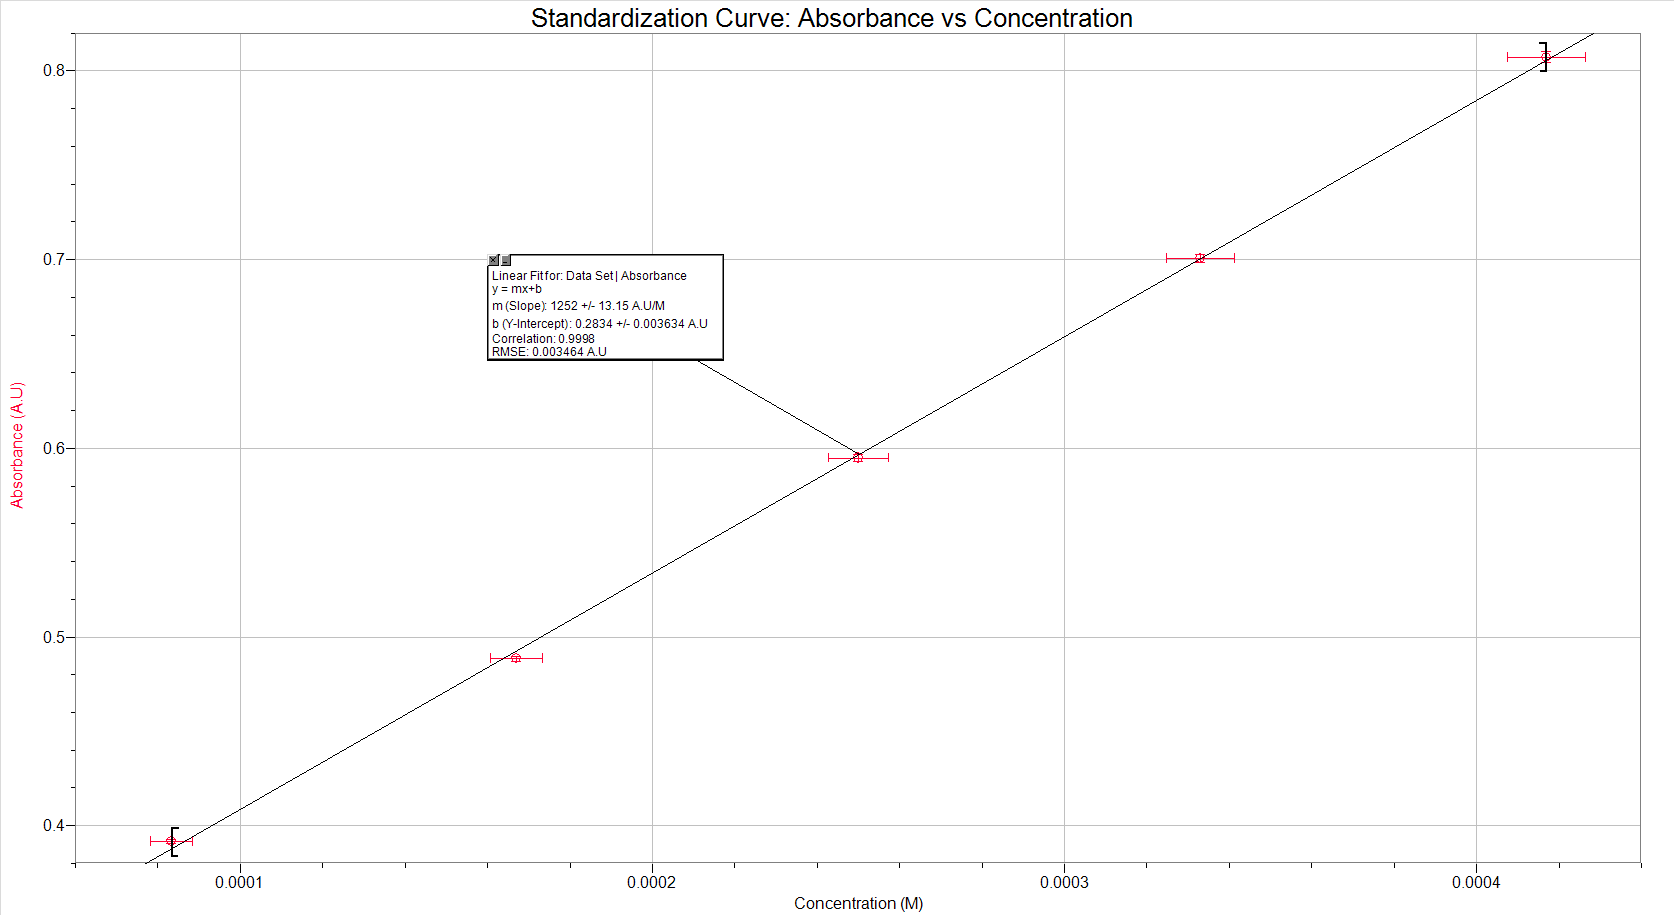
\includegraphics[width=100mm,height=\textheight,keepaspectratio]{images/standardization_curve.png}
    \caption{Standardization Curve: Absorbance vs Concentration}
    \label{fig:standardization_curve}
\end{figure}

\subsection{Relationship between Equilibrium Constant and Temperature}
To determine the relationship between the equilibrium constant and the temperature, I must derive the temperature and equilibrium constant. First, when dealing with temperature, it is important to ensure that the temperature is in Kelvin, so the zero point represents absolute zero. Therefore, the following formula must be applied. During the experiment, I noticed that the temperature was often \(\pm 1K\) of the true level temperature. Thus, rather than taking the uncertainty of the temperature sensor (\(\pm0.1K\)), I decided to take \(\pm 1K\) as the absolute uncertainty.

\begin{equation}
    T_K = T_C+273 = 25^\circ C + 273 = 298 \; K
\end{equation}

\noindent
To derive the equilibrium constant, I first calculated the initial concentrations of \(Fe^{3+}\) and \(SCN^-\). A sample calculation is shown below.

\begin{align}
    [Fe^{3+}]_{init} &= [Fe^{3+}]_{stock} \times V_{Fe^{3+}} = 0.0250 \; M \times 3.00 \; mL \times \frac{1}{45.0 \; mL} \\
    &= 1.67 \times 10^{-3} \; M \\
    [SCN^-]_{init} &= [SCN^-]_{stock} \times V_{SCN^-} = 0.0250 \; M \times 3.00 \; mL \times \frac{1}{45.0 \; mL} \\
    &= 1.67 \times 10^{-3} \; M
\end{align}

\noindent
Next, using \cref{eq:standardization_absorbance}, the absorbance can be derived from the transmittance. In \cref{fig:spectrophotometer_standardization}, the slope of Beer-Lambert Law curve was determined to be \(m=1252.26 \pm 13.15 \; M^{-1}\) and the intercept was determined to be \(b=0.2835 \pm 0.0036 \; AU\). Thus, the concentration of \(FeSCN^{2+}\) is:
\begin{equation}
    [FeSCN^{2+}]_{eq} = \frac{A - b}{m} = \frac{0.9337 \; AU
 - 0.2835 \; AU}{1252.26 \; M^{-1}} = 5.192 \times 10^{-4} \; M
\end{equation}

\begin{table}[H]
\centering
\begin{tabular}{l|ll|l}
  & \(Fe^{3+}\) & \(SCN^-\) & \(FeSCN^{2+}\) \\ \hline
  
I & \(1.67 \times 10^{-3}\)                      & \(1.67 \times 10^{-3}\)
                      & 0                      \\ 
C & \(-x\)                      & \(-x\)                      & \(+x\)                     \\ 
E & \((1.67 \times 10^{-3}) - x\)                      & \((1.67 \times 10^{-3}) - x\)                      & \(x\)                   \\ 
\end{tabular}
\caption{Concentration ICE for Given \([FeSCN^{2+}]_{eq}\)}
\label{table:ice_sample}
\end{table}

\noindent
The equilibrium constant can be calculated using the following formula. \cref{table:ice_sample} can be used to reduce the formula further.

\begin{align}
    K_c &= \frac{[FeSCN^{2+}]_{eq}}{[Fe^{3+}]_{eq} [SCN^-]_{eq}} \\
    &= \frac{[FeSCN^{2+}]_{eq}}{([Fe^{3+}]_{init} - [FeSCN^{2+}]_{eq}) \times ([SCN^-]_{init} - [FeSCN^{2+}]_{eq})} \\
    &= \frac{5.192 \times 10^{-4} \; M}{(1.67 \times 10^{-3} \; M - 5.192 \times 10^{-4} \; M) \times (1.67 \times 10^{-3} \; M - 5.192 \times 10^{-4} \; M)} \\
    &= 394
\end{align}

\noindent
The percent uncertainty of \(K_c\) can be estimated using the following formula. The conversion factors and concentration of the solutions are assumed to have negligible uncertainty.
\begin{align}
    \frac{\delta [Fe^{3+}]_{init}}{[Fe^{3+}]_{init}} &= \frac{0.05 \; mL}{3.00 \; mL} + \frac{0.2 \; mL}{45.0 \; mL} = 2\% \\
    \frac{\delta [SCN^-]_{init}}{[SCN^-]_{init}} &= \frac{0.05 \; mL}{3.00 \; mL} + \frac{0.2 \; mL}{45.0 \; mL} = 2\% \\
    \frac{\delta [FeSCN^{2+}]_{eq}}{[FeSCN^{2+}]_{eq}} &= \frac{0.0013 \; AU + 0.0036 \; AU}{0.6502 \; AU} + \frac{13.15 \; M^{-1}}{1252.26 \; M^{-1}} = 1.8\% \\
    \frac{\delta K_c}{K_c} &= \frac{\delta [FeSCN^{2+}]_{eq}}{[FeSCN^{2+}]_{eq}} + \frac{\delta [Fe^{3+}]_{eq}}{[Fe^{3+}]_{eq}} + \frac{\delta [SCN^-]_{eq}}{[SCN^-]_{eq}} \\
    &= 1.8 \% + \frac{4 \times 10^{-5} \; M}{1.15 \times 10^{-3} \; M} + \frac{4 \times 10^{-5} \; M}{1.15 \times 10^{-3} \; M} \\
    &= 10\%
\end{align}

\noindent
I repeated the above steps for each of the trials and levels in \cref{table:transmittance_temperature_data} to create \cref{table:before_linearization}. \cref{fig:before_linearization} is a plot of the equilibrium constant vs temperature data for the first trial. Similar results were found in the other trials.

\begin{table}[H]
\centering
\captionsetup{justification=centering,margin=2cm}
\resizebox{\textwidth}{!}{%
\begin{tabular}{|c|cccccccccccccc|}
\hline
\multirow{2}{*}{Temperature   (± 1K)} & \multicolumn{14}{c|}{Equilibrium   Constant}                                                                                                                                                                                                                                                                                                                                                                                                                                                                                                                                                                                        \\ \cline{2-15} 
                                      & \multicolumn{1}{c|}{Trial 1} & \multicolumn{1}{C{2.5cm}|}{Trial   1 Percent Uncertainty (\%)} & \multicolumn{1}{c|}{Trial   2} & \multicolumn{1}{C{2.5cm}|}{Trial   2 Percent Uncertainty (\%)} & \multicolumn{1}{c|}{Trial   3} & \multicolumn{1}{C{2.5cm}|}{Trial   3 Percent Uncertainty (\%)} & \multicolumn{1}{c|}{Trial   4} & \multicolumn{1}{C{2.5cm}|}{Trial   4 Percent Uncertainty (\%)} & \multicolumn{1}{c|}{Trial   5} & \multicolumn{1}{C{2.5cm}|}{Trial   5 Percent Uncertainty (\%)} & \multicolumn{1}{c|}{Trial   6} & \multicolumn{1}{C{2.5cm}|}{Trial   6 Percent Uncertainty (\%)} & \multicolumn{1}{c|}{Trial   7} & \multicolumn{1}{C{2.5cm}|}{Trial   7 Percent Uncertainty (\%)} \\ \hline
298                                   & \multicolumn{1}{c|}{394}     & \multicolumn{1}{c|}{10}                                 & \multicolumn{1}{c|}{391}       & \multicolumn{1}{c|}{10}                                 & \multicolumn{1}{c|}{374}       & \multicolumn{1}{c|}{10}                                 & \multicolumn{1}{c|}{374}       & \multicolumn{1}{c|}{10}                                 & \multicolumn{1}{c|}{402}       & \multicolumn{1}{c|}{10}                                 & \multicolumn{1}{c|}{404}       & \multicolumn{1}{c|}{10}                                 & \multicolumn{1}{c|}{373}       & 10                                 \\ \hline
303                                   & \multicolumn{1}{c|}{298}     & \multicolumn{1}{c|}{10}                                 & \multicolumn{1}{c|}{287}       & \multicolumn{1}{c|}{10}                                 & \multicolumn{1}{c|}{293}       & \multicolumn{1}{c|}{10}                                 & \multicolumn{1}{c|}{309}       & \multicolumn{1}{c|}{10}                                 & \multicolumn{1}{c|}{291}       & \multicolumn{1}{c|}{10}                                 & \multicolumn{1}{c|}{290}       & \multicolumn{1}{c|}{10}                                 & \multicolumn{1}{c|}{294}       & 10                                 \\ \hline
308                                   & \multicolumn{1}{c|}{253}     & \multicolumn{1}{c|}{10}                                 & \multicolumn{1}{c|}{234}       & \multicolumn{1}{c|}{10}                                 & \multicolumn{1}{c|}{237}       & \multicolumn{1}{c|}{10}                                 & \multicolumn{1}{c|}{251}       & \multicolumn{1}{c|}{10}                                 & \multicolumn{1}{c|}{236}       & \multicolumn{1}{c|}{10}                                 & \multicolumn{1}{c|}{248}       & \multicolumn{1}{c|}{10}                                 & \multicolumn{1}{c|}{252}       & 10                                 \\ \hline
313                                   & \multicolumn{1}{c|}{209}     & \multicolumn{1}{c|}{9}                                  & \multicolumn{1}{c|}{209}       & \multicolumn{1}{c|}{9}                                  & \multicolumn{1}{c|}{204}       & \multicolumn{1}{c|}{9}                                  & \multicolumn{1}{c|}{192}       & \multicolumn{1}{c|}{9}                                  & \multicolumn{1}{c|}{190}       & \multicolumn{1}{c|}{9}                                  & \multicolumn{1}{c|}{202}       & \multicolumn{1}{c|}{9}                                  & \multicolumn{1}{c|}{206}       & 9                                  \\ \hline
318                                   & \multicolumn{1}{c|}{176}     & \multicolumn{1}{c|}{9}                                  & \multicolumn{1}{c|}{179}       & \multicolumn{1}{c|}{9}                                  & \multicolumn{1}{c|}{179}       & \multicolumn{1}{c|}{9}                                  & \multicolumn{1}{c|}{173}       & \multicolumn{1}{c|}{9}                                  & \multicolumn{1}{c|}{171}       & \multicolumn{1}{c|}{9}                                  & \multicolumn{1}{c|}{173}       & \multicolumn{1}{c|}{9}                                  & \multicolumn{1}{c|}{167}       & 9                                  \\ \hline
323                                   & \multicolumn{1}{c|}{132}     & \multicolumn{1}{c|}{9}                                  & \multicolumn{1}{c|}{134}       & \multicolumn{1}{c|}{9}                                  & \multicolumn{1}{c|}{145}       & \multicolumn{1}{c|}{9}                                  & \multicolumn{1}{c|}{142}       & \multicolumn{1}{c|}{9}                                  & \multicolumn{1}{c|}{137}       & \multicolumn{1}{c|}{9}                                  & \multicolumn{1}{c|}{139}       & \multicolumn{1}{c|}{9}                                  & \multicolumn{1}{c|}{132}       & 9                                  \\ \hline
328                                   & \multicolumn{1}{c|}{114}     & \multicolumn{1}{c|}{9}                                  & \multicolumn{1}{c|}{114}       & \multicolumn{1}{c|}{9}                                  & \multicolumn{1}{c|}{117}       & \multicolumn{1}{c|}{9}                                  & \multicolumn{1}{c|}{111}       & \multicolumn{1}{c|}{9}                                  & \multicolumn{1}{c|}{113}       & \multicolumn{1}{c|}{9}                                  & \multicolumn{1}{c|}{104}       & \multicolumn{1}{c|}{9}                                  & \multicolumn{1}{c|}{113}       & 9                                  \\ \hline
333                                   & \multicolumn{1}{c|}{85.8}    & \multicolumn{1}{c|}{9}                                  & \multicolumn{1}{c|}{90.9}      & \multicolumn{1}{c|}{9}                                  & \multicolumn{1}{c|}{93.3}      & \multicolumn{1}{c|}{9}                                  & \multicolumn{1}{c|}{99.9}      & \multicolumn{1}{c|}{9}                                  & \multicolumn{1}{c|}{101}       & \multicolumn{1}{c|}{9}                                  & \multicolumn{1}{c|}{94.1}      & \multicolumn{1}{c|}{9}                                  & \multicolumn{1}{c|}{96.8}      & 9                                  \\ \hline
338                                   & \multicolumn{1}{c|}{74.3}    & \multicolumn{1}{c|}{9}                                  & \multicolumn{1}{c|}{79.5}      & \multicolumn{1}{c|}{9}                                  & \multicolumn{1}{c|}{87.3}      & \multicolumn{1}{c|}{9}                                  & \multicolumn{1}{c|}{75.1}      & \multicolumn{1}{c|}{9}                                  & \multicolumn{1}{c|}{83.9}      & \multicolumn{1}{c|}{9}                                  & \multicolumn{1}{c|}{82.2}      & \multicolumn{1}{c|}{9}                                  & \multicolumn{1}{c|}{85.5}      & 9                                  \\ \hline
343                                   & \multicolumn{1}{c|}{60.4}    & \multicolumn{1}{c|}{9}                                  & \multicolumn{1}{c|}{51.9}      & \multicolumn{1}{c|}{10}                                 & \multicolumn{1}{c|}{55.9}      & \multicolumn{1}{c|}{10}                                 & \multicolumn{1}{c|}{63.3}      & \multicolumn{1}{c|}{9}                                  & \multicolumn{1}{c|}{62.5}      & \multicolumn{1}{c|}{9}                                  & \multicolumn{1}{c|}{60.7}      & \multicolumn{1}{c|}{9}                                  & \multicolumn{1}{c|}{52.4}      & 10                                 \\ \hline
\end{tabular}}
\end{table}

\begin{table}[H]
\centering
\captionsetup{justification=centering,margin=2cm}
\resizebox{\textwidth}{!}{%
\begin{tabular}{|cccccccccccccc|}
\hline
\multicolumn{14}{|c|}{Equilibrium Constant (Continued.)}                                                                                                                                                                                                                                                                                                                                                                                                                                                                                                                                                                           \\ \hline
\multicolumn{1}{|c|}{Trial 8} & \multicolumn{1}{C{3cm}|}{Trial 8 Percent   Uncertainty (\%)} & \multicolumn{1}{c|}{Trial 9} & \multicolumn{1}{C{3cm}|}{Trial 9 Percent   Uncertainty (\%)} & \multicolumn{1}{c|}{Trial 10} & \multicolumn{1}{C{3cm}|}{Trial 10 Percent   Uncertainty (\%)} & \multicolumn{1}{c|}{Trial 11} & \multicolumn{1}{C{3cm}|}{Trial 11 Percent   Uncertainty (\%)} & \multicolumn{1}{c|}{Trial 12} & \multicolumn{1}{C{3cm}|}{Trial 12 Percent   Uncertainty (\%)} & \multicolumn{1}{c|}{Trial 13} & \multicolumn{1}{C{3cm}|}{Trial 13 Percent   Uncertainty (\%)} & \multicolumn{1}{c|}{Trial 14} & \multicolumn{1}{C{3cm}|}{Trial 14 Percent   Uncertainty (\%)} \\ \hline
\multicolumn{1}{|c|}{397}     & \multicolumn{1}{c|}{10}                                 & \multicolumn{1}{c|}{394}     & \multicolumn{1}{c|}{10}                                 & \multicolumn{1}{c|}{391}      & \multicolumn{1}{c|}{10}                                  & \multicolumn{1}{c|}{390}      & \multicolumn{1}{c|}{10}                                  & \multicolumn{1}{c|}{407}      & \multicolumn{1}{c|}{10}                                  & \multicolumn{1}{c|}{399}      & \multicolumn{1}{c|}{10}                                  & \multicolumn{1}{c|}{384}      & 10                                  \\ \hline
\multicolumn{1}{|c|}{287}     & \multicolumn{1}{c|}{10}                                 & \multicolumn{1}{c|}{288}     & \multicolumn{1}{c|}{10}                                 & \multicolumn{1}{c|}{296}      & \multicolumn{1}{c|}{10}                                  & \multicolumn{1}{c|}{307}      & \multicolumn{1}{c|}{10}                                  & \multicolumn{1}{c|}{290}      & \multicolumn{1}{c|}{10}                                  & \multicolumn{1}{c|}{298}      & \multicolumn{1}{c|}{10}                                  & \multicolumn{1}{c|}{293}      & 10                                  \\ \hline
\multicolumn{1}{|c|}{237}     & \multicolumn{1}{c|}{10}                                 & \multicolumn{1}{c|}{238}     & \multicolumn{1}{c|}{10}                                 & \multicolumn{1}{c|}{253}      & \multicolumn{1}{c|}{10}                                  & \multicolumn{1}{c|}{235}      & \multicolumn{1}{c|}{10}                                  & \multicolumn{1}{c|}{238}      & \multicolumn{1}{c|}{10}                                  & \multicolumn{1}{c|}{252}      & \multicolumn{1}{c|}{10}                                  & \multicolumn{1}{c|}{249}      & 10                                  \\ \hline
\multicolumn{1}{|c|}{213}     & \multicolumn{1}{c|}{9}                                  & \multicolumn{1}{c|}{205}     & \multicolumn{1}{c|}{9}                                  & \multicolumn{1}{c|}{193}      & \multicolumn{1}{c|}{9}                                   & \multicolumn{1}{c|}{204}      & \multicolumn{1}{c|}{9}                                   & \multicolumn{1}{c|}{205}      & \multicolumn{1}{c|}{9}                                   & \multicolumn{1}{c|}{211}      & \multicolumn{1}{c|}{9}                                   & \multicolumn{1}{c|}{215}      & 9                                   \\ \hline
\multicolumn{1}{|c|}{176}     & \multicolumn{1}{c|}{9}                                  & \multicolumn{1}{c|}{168}     & \multicolumn{1}{c|}{9}                                  & \multicolumn{1}{c|}{167}      & \multicolumn{1}{c|}{9}                                   & \multicolumn{1}{c|}{168}      & \multicolumn{1}{c|}{9}                                   & \multicolumn{1}{c|}{174}      & \multicolumn{1}{c|}{9}                                   & \multicolumn{1}{c|}{167}      & \multicolumn{1}{c|}{9}                                   & \multicolumn{1}{c|}{168}      & 9                                   \\ \hline
\multicolumn{1}{|c|}{137}     & \multicolumn{1}{c|}{9}                                  & \multicolumn{1}{c|}{130}     & \multicolumn{1}{c|}{9}                                  & \multicolumn{1}{c|}{133}      & \multicolumn{1}{c|}{9}                                   & \multicolumn{1}{c|}{133}      & \multicolumn{1}{c|}{9}                                   & \multicolumn{1}{c|}{131}      & \multicolumn{1}{c|}{9}                                   & \multicolumn{1}{c|}{130}      & \multicolumn{1}{c|}{9}                                   & \multicolumn{1}{c|}{133}      & 9                                   \\ \hline
\multicolumn{1}{|c|}{114}     & \multicolumn{1}{c|}{9}                                  & \multicolumn{1}{c|}{107}     & \multicolumn{1}{c|}{9}                                  & \multicolumn{1}{c|}{109}      & \multicolumn{1}{c|}{9}                                   & \multicolumn{1}{c|}{103}      & \multicolumn{1}{c|}{9}                                   & \multicolumn{1}{c|}{114}      & \multicolumn{1}{c|}{9}                                   & \multicolumn{1}{c|}{116}      & \multicolumn{1}{c|}{9}                                   & \multicolumn{1}{c|}{109}      & 9                                   \\ \hline
\multicolumn{1}{|c|}{94.6}    & \multicolumn{1}{c|}{9}                                  & \multicolumn{1}{c|}{96.1}    & \multicolumn{1}{c|}{9}                                  & \multicolumn{1}{c|}{96.1}     & \multicolumn{1}{c|}{9}                                   & \multicolumn{1}{c|}{95.1}     & \multicolumn{1}{c|}{9}                                   & \multicolumn{1}{c|}{103}      & \multicolumn{1}{c|}{9}                                   & \multicolumn{1}{c|}{100}      & \multicolumn{1}{c|}{9}                                   & \multicolumn{1}{c|}{99.5}     & 9                                   \\ \hline
\multicolumn{1}{|c|}{77.8}    & \multicolumn{1}{c|}{9}                                  & \multicolumn{1}{c|}{84.7}    & \multicolumn{1}{c|}{9}                                  & \multicolumn{1}{c|}{76.1}     & \multicolumn{1}{c|}{9}                                   & \multicolumn{1}{c|}{74.7}     & \multicolumn{1}{c|}{9}                                   & \multicolumn{1}{c|}{85.8}     & \multicolumn{1}{c|}{9}                                   & \multicolumn{1}{c|}{83.7}     & \multicolumn{1}{c|}{9}                                   & \multicolumn{1}{c|}{82.8}     & 9                                   \\ \hline
\multicolumn{1}{|c|}{52.9}    & \multicolumn{1}{c|}{10}                                 & \multicolumn{1}{c|}{56.1}    & \multicolumn{1}{c|}{10}                                 & \multicolumn{1}{c|}{50.8}     & \multicolumn{1}{c|}{10}                                  & \multicolumn{1}{c|}{56.7}     & \multicolumn{1}{c|}{10}                                  & \multicolumn{1}{c|}{63.6}     & \multicolumn{1}{c|}{9}                                   & \multicolumn{1}{c|}{61}       & \multicolumn{1}{c|}{9}                                   & \multicolumn{1}{c|}{54.9}     & 10                                  \\ \hline
\end{tabular}}
\caption{Equilibrium Constant vs Temperature}
\label{table:before_linearization}
\end{table}

\begin{figure}[H]
    \centering
    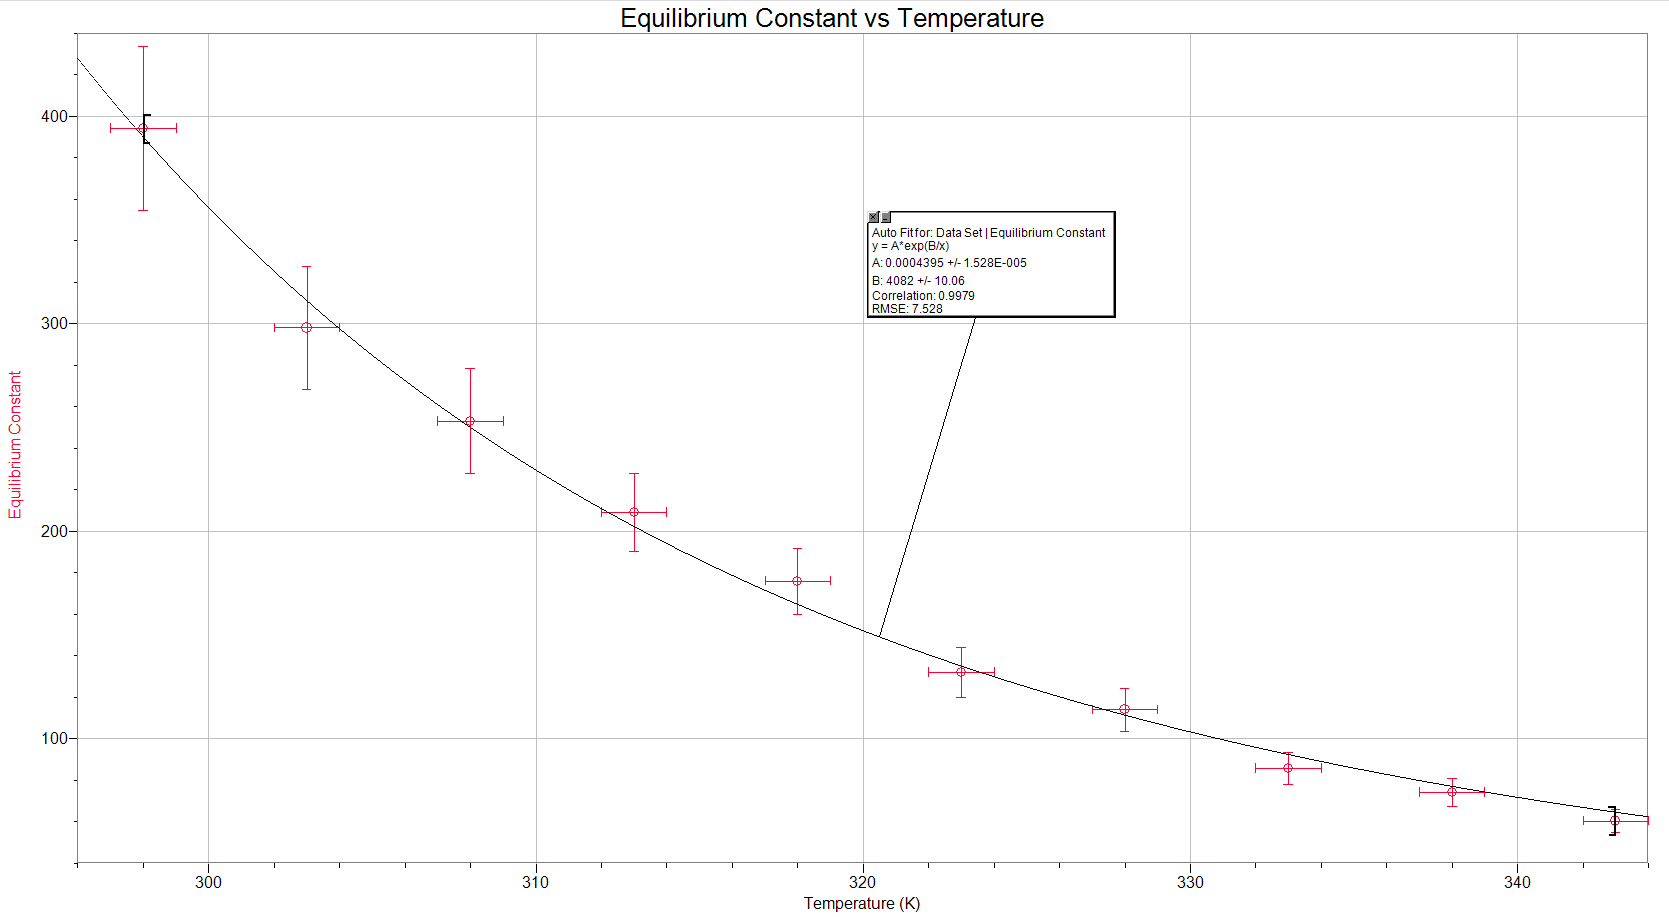
\includegraphics[width=100mm,height=\textheight,keepaspectratio]{images/before_linearization.png}
    \caption{Graph of Equilibrium Constant vs Temperature}
    \label{fig:before_linearization}
\end{figure}


\subsection{Linearization}
As seen in \cref{fig:before_linearization}, there is a very strong correlation (\(R^2=0.9979\)) to a \(K_c(T) = Ae^{B/T}\) curve, where A and B are coefficients. This matches the expected linearization as shown below.

\noindent
\newline
Setting the equations \(\Delta G^\circ = - RT\ln K_c\) and \(\Delta G^\circ = \Delta H^\circ - T \Delta S^\circ\) equal to each other.

\begin{align}
    - RT\ln K_c &= \Delta H^\circ - T \Delta S^\circ \\
    \ln K_c &= - \frac{\Delta H^\circ}{R} \times \frac{1}{T} + \frac{\Delta S^\circ}{R} \label{eq:linearization_theory}
\end{align}

\noindent
\cref{eq:linearization_theory} indicates that by taking the natural log of \(K_c\) and the reciprocal of temperature the relationship should be linear. A sample calculation is shown for this linearization.

\begin{equation}
    \textit{Reciprocal of Temperature} = \frac{1}{T_K} = \frac{1}{298 \; K} = 0.00336 K^{-1}
\end{equation}

\noindent
The uncertainty of \(\frac{1}{T_K}\) can be determined using \cref{eq:general_uncertainty}, 

\begin{align}
    \delta \left(\frac{1}{T_K}\right) &= \sqrt{\left(\frac{\partial \left(\frac{1}{T_K}\right)}{\partial T_K} \delta T_K \right)^2} = \frac{\delta T_K}{T^2} = \frac{1 \; K}{(298 \; K)^2} = 1 \times 10^{-5} \; K^{-1} \\
    \frac{\delta \left(\frac{1}{T_K}\right)}{\frac{1}{T_K}} &= 0.34\%
\end{align}

\noindent
Similarly,
\begin{equation}
    \textit{Natural Log of Equilibrium Constant} = \ln K_c = \ln 394 = 5.98
\end{equation}
\begin{align}
    \delta \ln K_c &= \sqrt{\left(\frac{\partial \ln K_c}{\partial T}\delta K_c \right)^2} = \frac{\delta K_c}{K_c} = \frac{37.59}{394} = 0.10 \\
    \frac{\delta \ln K_c}{\ln K_c} &= 1.8\%
\end{align}

\noindent
Repeating the above steps for each of the measurements to create \cref{table:after_linearization}.

\begin{table}[H]
\centering
\captionsetup{justification=centering,margin=2cm}
\resizebox{\textwidth}{!}{%
\begin{tabular}{|c|c|cccccccccccc|}
\hline
\multirow{2}{3cm}{\centering Reciprocal   of Temperature (1/K)} & \multirow{2}{4cm}{\centering Reciprocal of   Temperature Percent Uncertainty (\%)} & \multicolumn{12}{c|}{Natural Log of Equilibrium Constant}                                                                                                                                                                                                                                                                                                                                                                                                                                                                                \\ \cline{3-14} 
                                                   &                                                                       & \multicolumn{1}{c|}{Trial 1} & \multicolumn{1}{C{3cm}|}{Trial   1 Percent Uncertainty (\%)} & \multicolumn{1}{c|}{Trial   2} & \multicolumn{1}{C{3cm}|}{Trial   2 Percent Uncertainty (\%)} & \multicolumn{1}{c|}{Trial   3} & \multicolumn{1}{C{3cm}|}{Trial   3 Percent Uncertainty (\%)} & \multicolumn{1}{c|}{Trial   4} & \multicolumn{1}{C{3cm}|}{Trial   4 Percent Uncertainty (\%)} & \multicolumn{1}{c|}{Trial   5} & \multicolumn{1}{C{3cm}|}{Trial   5 Percent Uncertainty (\%)} & \multicolumn{1}{c|}{Trial   6} & \multicolumn{1}{C{3cm}|}{Trial   6 Percent Uncertainty (\%)} \\ \hline
0.00336                                            & 0.34                                                                  & \multicolumn{1}{c|}{5.98}    & \multicolumn{1}{c|}{1.8}                                & \multicolumn{1}{c|}{5.97}      & \multicolumn{1}{c|}{1.8}                                & \multicolumn{1}{c|}{5.92}      & \multicolumn{1}{c|}{1.7}                                & \multicolumn{1}{c|}{5.92}      & \multicolumn{1}{c|}{1.7}                                & \multicolumn{1}{c|}{6.00}      & \multicolumn{1}{c|}{1.8}                                & \multicolumn{1}{c|}{6.00}      & 1.8                                \\ \hline
0.00330                                            & 0.33                                                                  & \multicolumn{1}{c|}{5.70}    & \multicolumn{1}{c|}{1.7}                                & \multicolumn{1}{c|}{5.66}      & \multicolumn{1}{c|}{1.7}                                & \multicolumn{1}{c|}{5.68}      & \multicolumn{1}{c|}{1.7}                                & \multicolumn{1}{c|}{5.73}      & \multicolumn{1}{c|}{1.7}                                & \multicolumn{1}{c|}{5.67}      & \multicolumn{1}{c|}{1.7}                                & \multicolumn{1}{c|}{5.67}      & 1.7                                \\ \hline
0.00325                                            & 0.32                                                                  & \multicolumn{1}{c|}{5.53}    & \multicolumn{1}{c|}{1.7}                                & \multicolumn{1}{c|}{5.46}      & \multicolumn{1}{c|}{1.8}                                & \multicolumn{1}{c|}{5.47}      & \multicolumn{1}{c|}{1.8}                                & \multicolumn{1}{c|}{5.52}      & \multicolumn{1}{c|}{1.7}                                & \multicolumn{1}{c|}{5.46}      & \multicolumn{1}{c|}{1.8}                                & \multicolumn{1}{c|}{5.52}      & 1.7                                \\ \hline
0.00320                                            & 0.32                                                                  & \multicolumn{1}{c|}{5.34}    & \multicolumn{1}{c|}{1.8}                                & \multicolumn{1}{c|}{5.34}      & \multicolumn{1}{c|}{1.8}                                & \multicolumn{1}{c|}{5.32}      & \multicolumn{1}{c|}{1.8}                                & \multicolumn{1}{c|}{5.26}      & \multicolumn{1}{c|}{1.8}                                & \multicolumn{1}{c|}{5.25}      & \multicolumn{1}{c|}{1.8}                                & \multicolumn{1}{c|}{5.31}      & 1.8                                \\ \hline
0.00315                                            & 0.31                                                                  & \multicolumn{1}{c|}{5.17}    & \multicolumn{1}{c|}{1.8}                                & \multicolumn{1}{c|}{5.19}      & \multicolumn{1}{c|}{1.8}                                & \multicolumn{1}{c|}{5.19}      & \multicolumn{1}{c|}{1.8}                                & \multicolumn{1}{c|}{5.15}      & \multicolumn{1}{c|}{1.8}                                & \multicolumn{1}{c|}{5.14}      & \multicolumn{1}{c|}{1.8}                                & \multicolumn{1}{c|}{5.15}      & 1.8                                \\ \hline
0.00310                                            & 0.31                                                                  & \multicolumn{1}{c|}{4.88}    & \multicolumn{1}{c|}{1.9}                                & \multicolumn{1}{c|}{4.90}      & \multicolumn{1}{c|}{1.9}                                & \multicolumn{1}{c|}{4.98}      & \multicolumn{1}{c|}{1.8}                                & \multicolumn{1}{c|}{4.96}      & \multicolumn{1}{c|}{1.8}                                & \multicolumn{1}{c|}{4.92}      & \multicolumn{1}{c|}{1.9}                                & \multicolumn{1}{c|}{4.94}      & 1.9                                \\ \hline
0.00305                                            & 0.30                                                                  & \multicolumn{1}{c|}{4.73}    & \multicolumn{1}{c|}{1.9}                                & \multicolumn{1}{c|}{4.74}      & \multicolumn{1}{c|}{1.9}                                & \multicolumn{1}{c|}{4.76}      & \multicolumn{1}{c|}{1.9}                                & \multicolumn{1}{c|}{4.71}      & \multicolumn{1}{c|}{1.9}                                & \multicolumn{1}{c|}{4.73}      & \multicolumn{1}{c|}{1.9}                                & \multicolumn{1}{c|}{4.65}      & 2.0                                \\ \hline
0.00300                                            & 0.30                                                                  & \multicolumn{1}{c|}{4.45}    & \multicolumn{1}{c|}{2.0}                                & \multicolumn{1}{c|}{4.51}      & \multicolumn{1}{c|}{2.0}                                & \multicolumn{1}{c|}{4.54}      & \multicolumn{1}{c|}{2.0}                                & \multicolumn{1}{c|}{4.60}      & \multicolumn{1}{c|}{2.0}                                & \multicolumn{1}{c|}{4.62}      & \multicolumn{1}{c|}{2.0}                                & \multicolumn{1}{c|}{4.54}      & 2.0                                \\ \hline
0.00296                                            & 0.30                                                                  & \multicolumn{1}{c|}{4.31}    & \multicolumn{1}{c|}{2.0}                                & \multicolumn{1}{c|}{4.38}      & \multicolumn{1}{c|}{2.0}                                & \multicolumn{1}{c|}{4.47}      & \multicolumn{1}{c|}{2.0}                                & \multicolumn{1}{c|}{4.32}      & \multicolumn{1}{c|}{2.0}                                & \multicolumn{1}{c|}{4.43}      & \multicolumn{1}{c|}{2.0}                                & \multicolumn{1}{c|}{4.41}      & 2.0                                \\ \hline
0.00292                                            & 0.29                                                                  & \multicolumn{1}{c|}{4.10}    & \multicolumn{1}{c|}{2.0}                                & \multicolumn{1}{c|}{3.95}      & \multicolumn{1}{c|}{2.0}                                & \multicolumn{1}{c|}{4.02}      & \multicolumn{1}{c|}{2.0}                                & \multicolumn{1}{c|}{4.15}      & \multicolumn{1}{c|}{2.0}                                & \multicolumn{1}{c|}{4.13}      & \multicolumn{1}{c|}{2.0}                                & \multicolumn{1}{c|}{4.11}      & 2.0                                \\ \hline
\end{tabular}}
\end{table}

\begin{table}[H]
\centering
\captionsetup{justification=centering,margin=1cm}
\resizebox{\textwidth}{!}{%
\begin{tabular}{|cccccccccccccccc|}
\hline
\multicolumn{16}{|c|}{Natural Log of Equilibrium Constant (Continued.)}                                                                                                                                                                                                                                                                                                                                                                                                                                                                                                                                                            \\ \hline \multicolumn{1}{|c|}{Trial 7} & \multicolumn{1}{C{3cm}|}{Trial 7 Percent   Uncertainty (\%)} & \multicolumn{1}{|c|}{Trial 8} & \multicolumn{1}{C{3cm}|}{Trial 8 Percent   Uncertainty (\%)} & \multicolumn{1}{c|}{Trial 9} & \multicolumn{1}{C{3cm}|}{Trial 9 Percent   Uncertainty (\%)} & \multicolumn{1}{c|}{Trial 10} & \multicolumn{1}{C{3cm}|}{Trial 10   Percent Uncertainty (\%)} & \multicolumn{1}{c|}{Trial 11} & \multicolumn{1}{C{3cm}|}{Trial 11   Percent Uncertainty (\%)} & \multicolumn{1}{c|}{Trial 12} & \multicolumn{1}{C{3cm}|}{Trial 12   Percent Uncertainty (\%)} & \multicolumn{1}{c|}{Trial 13} & \multicolumn{1}{C{3cm}|}{Trial 13   Percent Uncertainty (\%)} & \multicolumn{1}{c|}{Trial 14} & \multicolumn{1}{C{3cm}|}{Trial 14   Percent Uncertainty (\%)} \\ \hline
\multicolumn{1}{|c|}{5.92}    & \multicolumn{1}{c|}{1.7}                                & \multicolumn{1}{c|}{5.98}    & \multicolumn{1}{c|}{1.8}                                & \multicolumn{1}{c|}{5.98}    & \multicolumn{1}{c|}{1.8}                                & \multicolumn{1}{c|}{5.97}     & \multicolumn{1}{c|}{1.8}                                 & \multicolumn{1}{c|}{5.97}     & \multicolumn{1}{c|}{1.8}                                 & \multicolumn{1}{c|}{6.01}     & \multicolumn{1}{c|}{1.8}                                 & \multicolumn{1}{c|}{5.99}     & \multicolumn{1}{c|}{1.8}                                 & \multicolumn{1}{c|}{5.95}     & 1.7                                 \\ \hline
\multicolumn{1}{|c|}{5.68}    & \multicolumn{1}{c|}{1.7}                                & \multicolumn{1}{c|}{5.66}    & \multicolumn{1}{c|}{1.7}                                & \multicolumn{1}{c|}{5.66}    & \multicolumn{1}{c|}{1.7}                                & \multicolumn{1}{c|}{5.69}     & \multicolumn{1}{c|}{1.7}                                 & \multicolumn{1}{c|}{5.73}     & \multicolumn{1}{c|}{1.7}                                 & \multicolumn{1}{c|}{5.67}     & \multicolumn{1}{c|}{1.7}                                 & \multicolumn{1}{c|}{5.70}     & \multicolumn{1}{c|}{1.7}                                 & \multicolumn{1}{c|}{5.68}     & 1.7                                 \\ \hline
\multicolumn{1}{|c|}{5.53}    & \multicolumn{1}{c|}{1.7}                                & \multicolumn{1}{c|}{5.47}    & \multicolumn{1}{c|}{1.8}                                & \multicolumn{1}{c|}{5.47}    & \multicolumn{1}{c|}{1.8}                                & \multicolumn{1}{c|}{5.53}     & \multicolumn{1}{c|}{1.7}                                 & \multicolumn{1}{c|}{5.46}     & \multicolumn{1}{c|}{1.8}                                 & \multicolumn{1}{c|}{5.47}     & \multicolumn{1}{c|}{1.8}                                 & \multicolumn{1}{c|}{5.53}     & \multicolumn{1}{c|}{1.7}                                 & \multicolumn{1}{c|}{5.52}     & 1.7                                 \\ \hline
\multicolumn{1}{|c|}{5.33}    & \multicolumn{1}{c|}{1.8}                                & \multicolumn{1}{c|}{5.36}    & \multicolumn{1}{c|}{1.8}                                & \multicolumn{1}{c|}{5.32}    & \multicolumn{1}{c|}{1.8}                                & \multicolumn{1}{c|}{5.26}     & \multicolumn{1}{c|}{1.8}                                 & \multicolumn{1}{c|}{5.32}     & \multicolumn{1}{c|}{1.8}                                 & \multicolumn{1}{c|}{5.32}     & \multicolumn{1}{c|}{1.8}                                 & \multicolumn{1}{c|}{5.35}     & \multicolumn{1}{c|}{1.8}                                 & \multicolumn{1}{c|}{5.37}     & 1.8                                 \\ \hline
\multicolumn{1}{|c|}{5.12}    & \multicolumn{1}{c|}{1.8}                                & \multicolumn{1}{c|}{5.17}    & \multicolumn{1}{c|}{1.8}                                & \multicolumn{1}{c|}{5.13}    & \multicolumn{1}{c|}{1.8}                                & \multicolumn{1}{c|}{5.12}     & \multicolumn{1}{c|}{1.8}                                 & \multicolumn{1}{c|}{5.13}     & \multicolumn{1}{c|}{1.8}                                 & \multicolumn{1}{c|}{5.16}     & \multicolumn{1}{c|}{1.8}                                 & \multicolumn{1}{c|}{5.12}     & \multicolumn{1}{c|}{1.8}                                 & \multicolumn{1}{c|}{5.13}     & 1.8                                 \\ \hline
\multicolumn{1}{|c|}{4.88}    & \multicolumn{1}{c|}{1.9}                                & \multicolumn{1}{c|}{4.92}    & \multicolumn{1}{c|}{1.9}                                & \multicolumn{1}{c|}{4.87}    & \multicolumn{1}{c|}{1.9}                                & \multicolumn{1}{c|}{4.89}     & \multicolumn{1}{c|}{1.9}                                 & \multicolumn{1}{c|}{4.89}     & \multicolumn{1}{c|}{1.9}                                 & \multicolumn{1}{c|}{4.88}     & \multicolumn{1}{c|}{1.9}                                 & \multicolumn{1}{c|}{4.87}     & \multicolumn{1}{c|}{1.9}                                 & \multicolumn{1}{c|}{4.89}     & 1.9                                 \\ \hline
\multicolumn{1}{|c|}{4.73}    & \multicolumn{1}{c|}{1.9}                                & \multicolumn{1}{c|}{4.74}    & \multicolumn{1}{c|}{1.9}                                & \multicolumn{1}{c|}{4.67}    & \multicolumn{1}{c|}{1.9}                                & \multicolumn{1}{c|}{4.69}     & \multicolumn{1}{c|}{1.9}                                 & \multicolumn{1}{c|}{4.64}     & \multicolumn{1}{c|}{2.0}                                 & \multicolumn{1}{c|}{4.74}     & \multicolumn{1}{c|}{1.9}                                 & \multicolumn{1}{c|}{4.75}     & \multicolumn{1}{c|}{1.9}                                 & \multicolumn{1}{c|}{4.69}     & 1.9                                 \\ \hline
\multicolumn{1}{|c|}{4.57}    & \multicolumn{1}{c|}{2.0}                                & \multicolumn{1}{c|}{4.55}    & \multicolumn{1}{c|}{2.0}                                & \multicolumn{1}{c|}{4.57}    & \multicolumn{1}{c|}{2.0}                                & \multicolumn{1}{c|}{4.57}     & \multicolumn{1}{c|}{2.0}                                 & \multicolumn{1}{c|}{4.56}     & \multicolumn{1}{c|}{2.0}                                 & \multicolumn{1}{c|}{4.64}     & \multicolumn{1}{c|}{2.0}                                 & \multicolumn{1}{c|}{4.61}     & \multicolumn{1}{c|}{2.0}                                 & \multicolumn{1}{c|}{4.60}     & 2.0                                 \\ \hline
\multicolumn{1}{|c|}{4.45}    & \multicolumn{1}{c|}{2.0}                                & \multicolumn{1}{c|}{4.35}    & \multicolumn{1}{c|}{2.0}                                & \multicolumn{1}{c|}{4.44}    & \multicolumn{1}{c|}{2.0}                                & \multicolumn{1}{c|}{4.33}     & \multicolumn{1}{c|}{2.0}                                 & \multicolumn{1}{c|}{4.31}     & \multicolumn{1}{c|}{2.0}                                 & \multicolumn{1}{c|}{4.45}     & \multicolumn{1}{c|}{2.0}                                 & \multicolumn{1}{c|}{4.43}     & \multicolumn{1}{c|}{2.0}                                 & \multicolumn{1}{c|}{4.42}     & 2.0                                 \\ \hline
\multicolumn{1}{|c|}{3.96}    & \multicolumn{1}{c|}{2.0}                                & \multicolumn{1}{c|}{3.97}    & \multicolumn{1}{c|}{2.0}                                & \multicolumn{1}{c|}{4.03}    & \multicolumn{1}{c|}{2.0}                                & \multicolumn{1}{c|}{3.93}     & \multicolumn{1}{c|}{2.0}                                 & \multicolumn{1}{c|}{4.04}     & \multicolumn{1}{c|}{2.0}                                 & \multicolumn{1}{c|}{4.15}     & \multicolumn{1}{c|}{2.0}                                 & \multicolumn{1}{c|}{4.11}     & \multicolumn{1}{c|}{2.0}                                 & \multicolumn{1}{c|}{4.01}     & 2.0                                 \\ \hline
\end{tabular}}
\caption{Natural Log of Equilibrium Constant vs Reciprocal of Temperature}
\label{table:after_linearization}
\end{table}

Finally, the average natural log of the equilibrium constant was determined for each of the reciprocal of temperature levels. The uncertainty of this average can be determined using the following formula. A sample calculation is shown below.

\begin{align}
    \delta (\ln K_c)_{avg} &= \frac{(\ln K_c)_{max} - (\ln K_c)_{min}}{2\sqrt{N}} = \frac{6.01 - 5.92}{2\sqrt{14}} = 0.01 \\
    \frac{\delta (\ln K_c)_{avg}}{(\ln K_c)_{avg}} &= 0.19\%
\end{align}

\noindent
Performing the average calculation for each reciprocal of temperature level, I created \cref{table:after_linearization_avg} and \cref{fig:after_linearization}.

\begin{table}[H]
\centering
\begin{tabular}{|c|c|c|c|}
\hline
\multicolumn{1}{|C{2.5cm}|}{Reciprocal   of Temperature (1/K)} & \multicolumn{1}{|C{4cm}|}{Reciprocal of   Temperature Percent Uncertainty (\%)} & \multicolumn{1}{|C{3.5cm}|}{Average Natural   Log of Equilibrium Constant} & \multicolumn{1}{|C{5cm}|}{Average Natural   Log of Equilibrium Constant Percent Uncertainty (\%)} \\ \hline
0.00336                           & 0.34                                                 & 5.97                                          & 0.19                                                                   \\ \hline
0.00330                           & 0.33                                                 & 5.68                                          & 0.18                                                                   \\ \hline
0.00325                           & 0.32                                                 & 5.50                                          & 0.19                                                                   \\ \hline
0.00320                           & 0.32                                                 & 5.32                                          & 0.31                                                                   \\ \hline
0.00315                           & 0.31                                                 & 5.15                                          & 0.17                                                                   \\ \hline
0.00310                           & 0.31                                                 & 4.90                                          & 0.30                                                                   \\ \hline
0.00305                           & 0.30                                                 & 4.71                                          & 0.36                                                                   \\ \hline
0.00300                           & 0.30                                                 & 4.57                                          & 0.55                                                                   \\ \hline
0.00296                           & 0.30                                                 & 4.39                                          & 0.49                                                                   \\ \hline
0.00292                           & 0.29                                                 & 4.05                                          & 0.73                                                                   \\ \hline
\end{tabular}
\caption{Average Natural Log of Equilibrium Constant vs Reciprocal of Temperature}
\label{table:after_linearization_avg}
\end{table}

\begin{figure}[H]
    \centering
    \captionsetup{justification=centering,margin=1.5cm}
    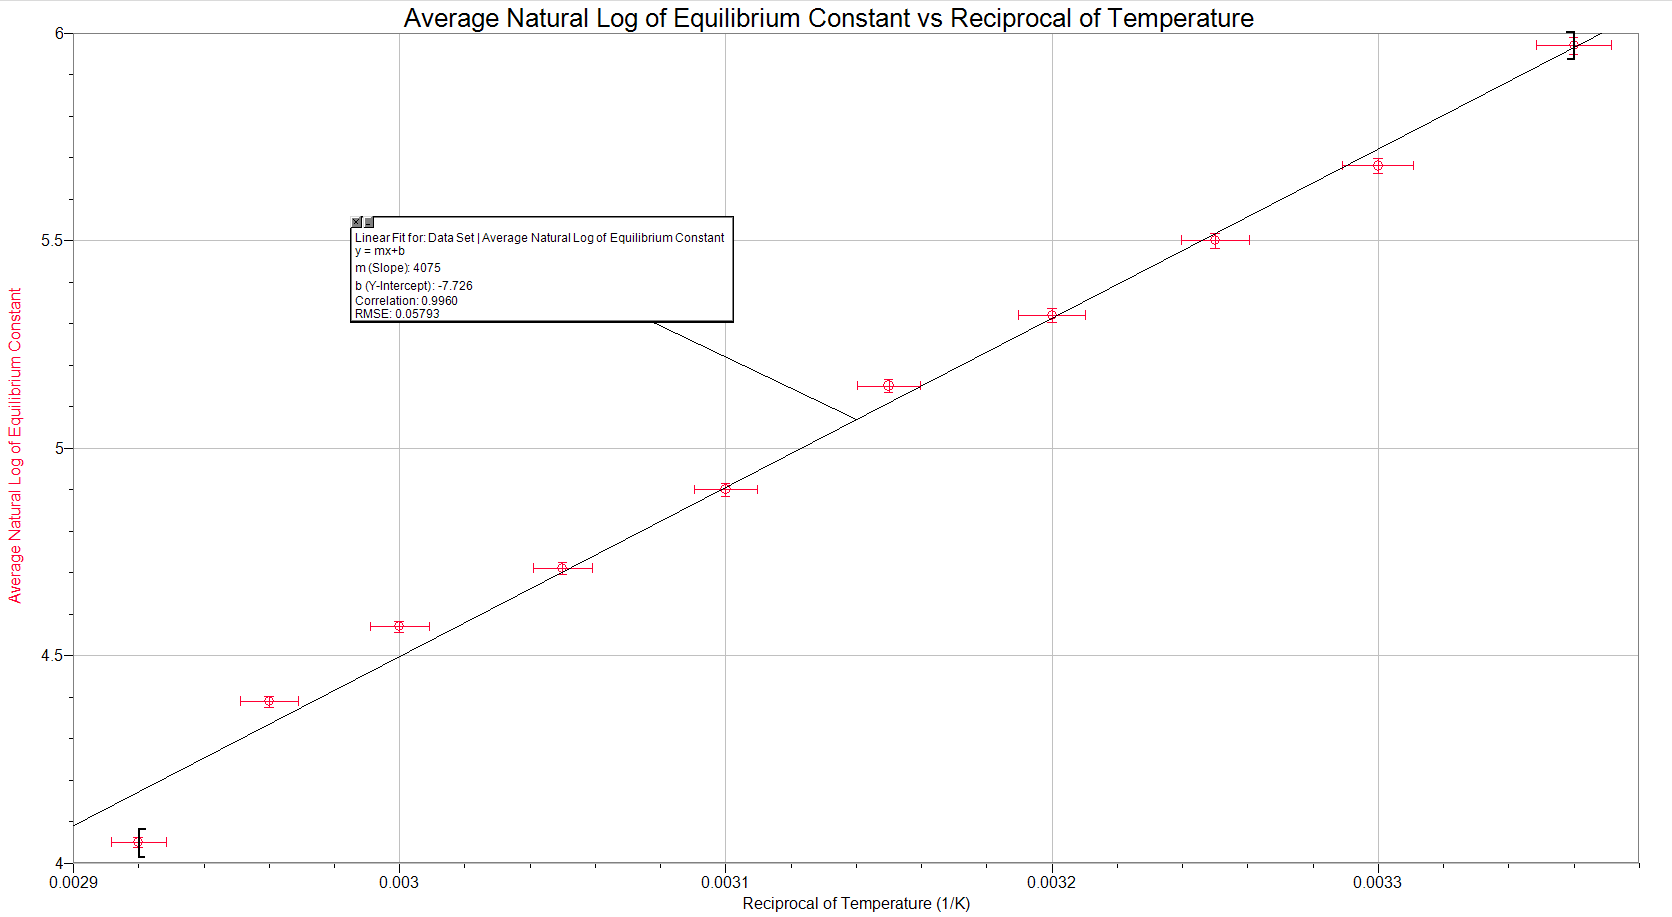
\includegraphics[width=100mm,height=\textheight,keepaspectratio]{images/after_linearization.png}
    \caption{Graph of Average Natural Log of Equilibrium Constant vs Reciprocal of Temperature}
    \label{fig:after_linearization}
\end{figure}

% \subsection{Percent Uncertainty and Percent Error of Slope}
% A rough estimate of the percent uncertainty of the slope $\beta$ can be determined by utilizing the maximum and minimum slope lines.
% \[\delta \beta = \frac{\beta_{max}-\beta_{min}}{2} = \frac{3719 K \ln{k\Omega}-3335 K \ln{k\Omega}}{2}=192 K \ln{k\Omega}\]
% \[\frac{\delta \beta}{\beta}=\frac{192 K \ln{k\Omega}}{3556 K \ln{k\Omega}}=5.40 \%\]

% The accepted value for the slope $\beta$ for this NTC Themistor is $3474 K \ln{k\Omega}$.
% Therefore, to calculate the percent error, the following calculation can be performed.
% \[Percent \; Error = \frac{|\beta_{actual} - \beta_{accepted}|}{\beta_{accepted}}=\frac{|3556 K \ln{k\Omega} - 3474 K \ln{k\Omega}|}{3474 K \ln{k\Omega}}=2.36\%\]


\subsection{Interpretation}
As seen in \cref{fig:after_linearization}), the line of best fit indicates a positive linear relationship between \(\ln K_c\) and \(\frac{1}{T}\). This means as \(\frac{1}{T}\) increases, \(\ln{K_c}\) will increase proportionally. Thus, this linearization proves that there is a negative exponential relationship between \(K_c\) and \(T\).

There is a very strong correlation (\(R^2=0.9960\)) between the linear regression and the linearized data. The line of best fit passes through almost all points and uncertainty bars. The minimum and maximum slope lines are very similar to the regression line. All this affirms that the \(K_c\) and \(T\) of a thiocynatoiron complex reaction follow a negative exponential relationship.

Finally, the slope and intercept of this linearized graph is proportional to the standard enthalpy change and entropy change of the reaction respectively, as shown in \cref{eq:linearization_theory}. Thus, the formation of the thiocynatoiron complex is exothermic and decreases entropy. The small \(\Delta H^\circ\) and \(\Delta S^\circ\) may be due to the formation of weak coordinate covalent bonds in the thiocyanatoiron complex.

\begin{align}
    \Delta H^\circ &= - m \times R = - 4075\; K \times 8.314 \; J \; mol^{-1} \; K^{-1} = -33880 \; J \; mol^{-1} \\
    \Delta S^\circ &= b \times R = -7.726 \times 8.314 \; J \; mol^{-1} \; K^{-1} = -64.23 \; J \; mol^{-1} \; K^{-1}
\end{align}

\section{Conclusion}
Therefore, according to this experiment, there is a very strong correlation (\(R^2=0.9960\)) for a negative exponential relationship between the equilibrium constant and the temperature of a thiocyanatoiron complex reaction.
This matches my hypothesis for this experiment. Furthermore, the individual trial percent uncertainties was far below 5\%, which means that my measurement system is precise. The average percent uncertainties were also far below 5\% which means that the experiment had a precise procedure. Finally, the derived enthalpy and entropy change was well within the accepted range, suggesting fairly accurate results throughout.

\section{Sources for Error}
Error could have been introduced from 4 sources: measurement of temperature using the Vernier Temperature Probe, measurement of transmittance using the spectrophotometer, the indirect heating of the cuvettes using a water bath, and temperature variations during the procedure.

First, the measurement of temperature using the Vernier Temperature Probe contributes to random error since the device uncertainty for the probe is \(\pm\;0.1 \; K\). The random error from this source is negligible in this experiment. Next, the measurement of transmittance using the spectrophotometer also contributes to random error since the device uncertainty for the device is \(\pm\;0.00035\). The random error from this source is also negligible in this experiment. Then, since the cuvettes was indirectly heated through a water bath, the temperature of the water could have been higher than that of the cuvettes leading to systematic error. However, since the heating was put on the lowest setting and the temperature of the cuvettes and the heat bath was normalized by waiting 2-3 minutes, the temperature of the cuvettes should have been relatively close to the temperature of the water bath. Hence, the systematic error from this source is negligible. Finally, as I removed the cuvettes from the hot water bath, wiped off the water on the surface, and placed the sample in the spectrophotometer, the temperature of the small sample likely changed fairly dramatically. This would contribute to a significant systematic error. To account for this, I increased my temperature uncertainty to \(\pm\;1\; K\).

In conclusion, most sources of error were minimal or well-accounted for throughout the experiment.

\section{Strengths}
One strength of this experiment is the use of the spectrophotometer to measure the concentration of the colored \(FeSCN^{2+}\) complex. Other methods to measure the concentration like titration would have taken much longer to complete. Since the spectrophotometer could measure the concentration in a few seconds, minimal temperature was lost from the cuvettes. Furthermore, the ability to take fast measurements enabled me to take a large number of trials and temperature levels. Thus, the use of the spectrophotometer significantly improved the accuracy and precision of this experiment. Another major strength of this experiment was the use of multiple cuvettes in the hot water bath. This allowed me to take all the transmittance measurements for a temperature level at the same time, greatly improving the speed of the experiment. Furthermore, when cuvettes were removed from the water bath, they would decrease in temperature slightly. However, by cycling through the cuvettes, each cuvette has enough time to return to the temperature of the hot water bath. 

\section{Weaknesses}
One weakness of this experiment was the drop in temperature of the cuvettes, while the measurement was taken. Though the measurement time was limited, the drop in temperature was still significant. Another weakness of this experiment was maintaining a consistent temperature for the water bath. Though the hot plate held the temperature relatively constant, it deviated by \(\pm 1^\circ C\), significantly increasing the random error and thus the percent uncertainty in the temperature. These were major experiment design flaws that need to be revised for future trials.

\section{Improvements}
Multiple improvements could be applied to this experiment to address its weaknesses. First, the use of cuvettes made of a more thermally insulating material could reduce the magnitude of the temperature drop. Furthermore, a correction factor could also be developed to adjust the measurements for the impact of temperature drop. Second, the volume of the water bath could be increased. Though it would take a longer period to heat the bath, it would also take a longer period for the bath to cool down. This would greatly diminish the random error from the fluctuating temperature and thus decrease the temperature percent uncertainty. These improvements would greatly improve both the accuracy and precision of this experiment.

\section{Extensions}
A possible extension to this experiment that might be worthy of future study is the relationship between the equilibrium constant and pressure. This experiment explored the relationship between the equilibrium constant and temperature as described by the Van 't Hoff Equation. However, in industrial processes, temperature is modulated along with pressure to achieve ideal operating conditions. Thus, understanding the precise relationship between the equilibrium constant and pressure is significant.


\newpage
\bibliography{ref}
\bibliographystyle{apalike}

\end{document}
